\chapter{The WisSim toolkit}\label{chapter5}
The WisSim is a visual WIreless Sensor network SIMulation toolkit, which was developed by researchers at SEDIC Lab \cite{sedic} for building a software tool that could help researchers and algorithm designers to test their newly proposed algorithms for wireless sensor networks. 

The WiSSim architecture follows the Client-Server architecture where at the client side it provides the front-end components for the user to define the test networks, algorithms and execution scripts, and possibly ask for simulation then run the visualization and analysis tools to enjoy seeing the test analysis results provided with care towards the user convenience and deep understanding. At the back-end, it exploits a popular existing network simulator software, that is \emph{ns-2}. The WiSSim server acts as a connector to work with \emph{ns-2}: preparing the Tcl scripts to be executed in \emph{ns-2} and retrieving and interpreting the trace files outputted from \emph{ns-2}. Besides WisSim server also implements into the \emph{ns-2} core certain selected routing protocols \cite{sedic}.

The remaining of this chapter describes an overview of \emph{ns-2} simulator and some features which have been implemented in WisSim client by the author.

\section{ns-2 simulator overview}
The \emph{ns-2} is a discrete-event simulation framework, which was developed by researchers at UC Berkeley from 1995. The general architecture of \emph{ns-2} is presented in figure \ref{fig-ns2-arch}. 
\begin{figure}[!htb]
\centering
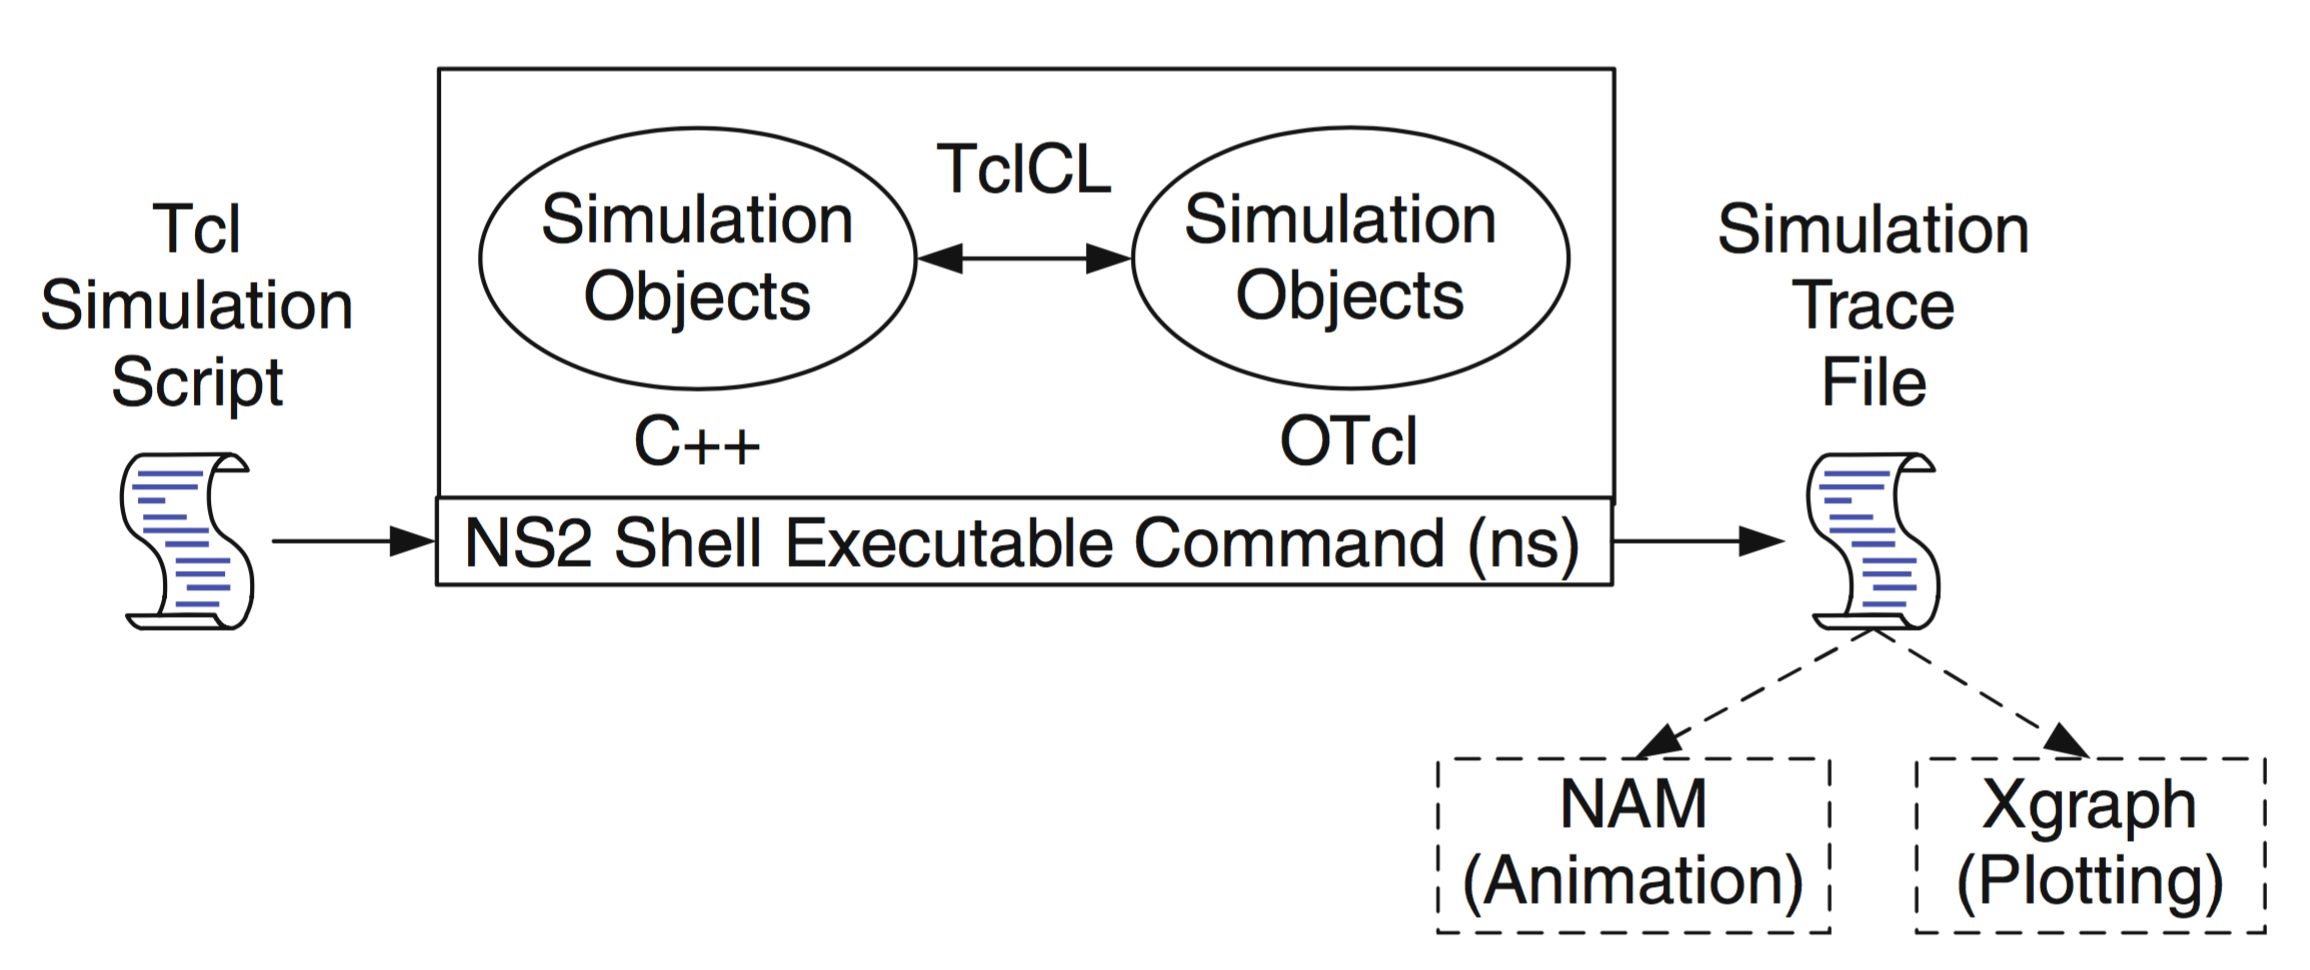
\includegraphics[width=0.6\textwidth]{Chapter5/Chapter5Figs/fig-ns2-arch.png}
\caption{The architecture of \emph{ns-2}.}
\label{fig-ns2-arch}
\end{figure} 

The simulation script is written in Tcl language. A simulation script must have:
\begin{itemize}
\item Network topology including network's size, number of sensor nodes, the configuration of each sensor nodes, network infrastructure, network protocol, and simulation time.
\item Declaration of events: the start time of the event, type of events, events' commands ...
\item Output format.
\end{itemize}
The output of simulation process called trace files. By analyzing these trace files, we can calculate network's metrics such as energy consumption, drop ratio or average path length, ...

The \emph{ns-2} uses two programming language: Tcl and C++. All the routing algorithms which are deployed into \emph{ns-2} core must be written in C++. The component of \emph{ns-2} could be classified into 4 groups based on their principal functions:
\begin{itemize}
\item Simulation-related Objects: controls and manages the simulation time. These objects are events, handlers, scheduler and simulator.
\item Network Objects: manages packet (transmit, receive, or drop).
\item Packet-related Objects: includes supporting packets.
\item Helper Objects: such as a routing protocol.
\end{itemize} 
As mentioned above, the \emph{ns-2} is a discrete-event simulation framework. More particularly, each event contains the time it will execute, its tasks and the link to the next event. These events create an event-chain, that is a single linked list and is created during the simulation process. Figure \ref{fig-ns2-event} shows an example of event-chain. 
\begin{figure}[!htb]
\centering
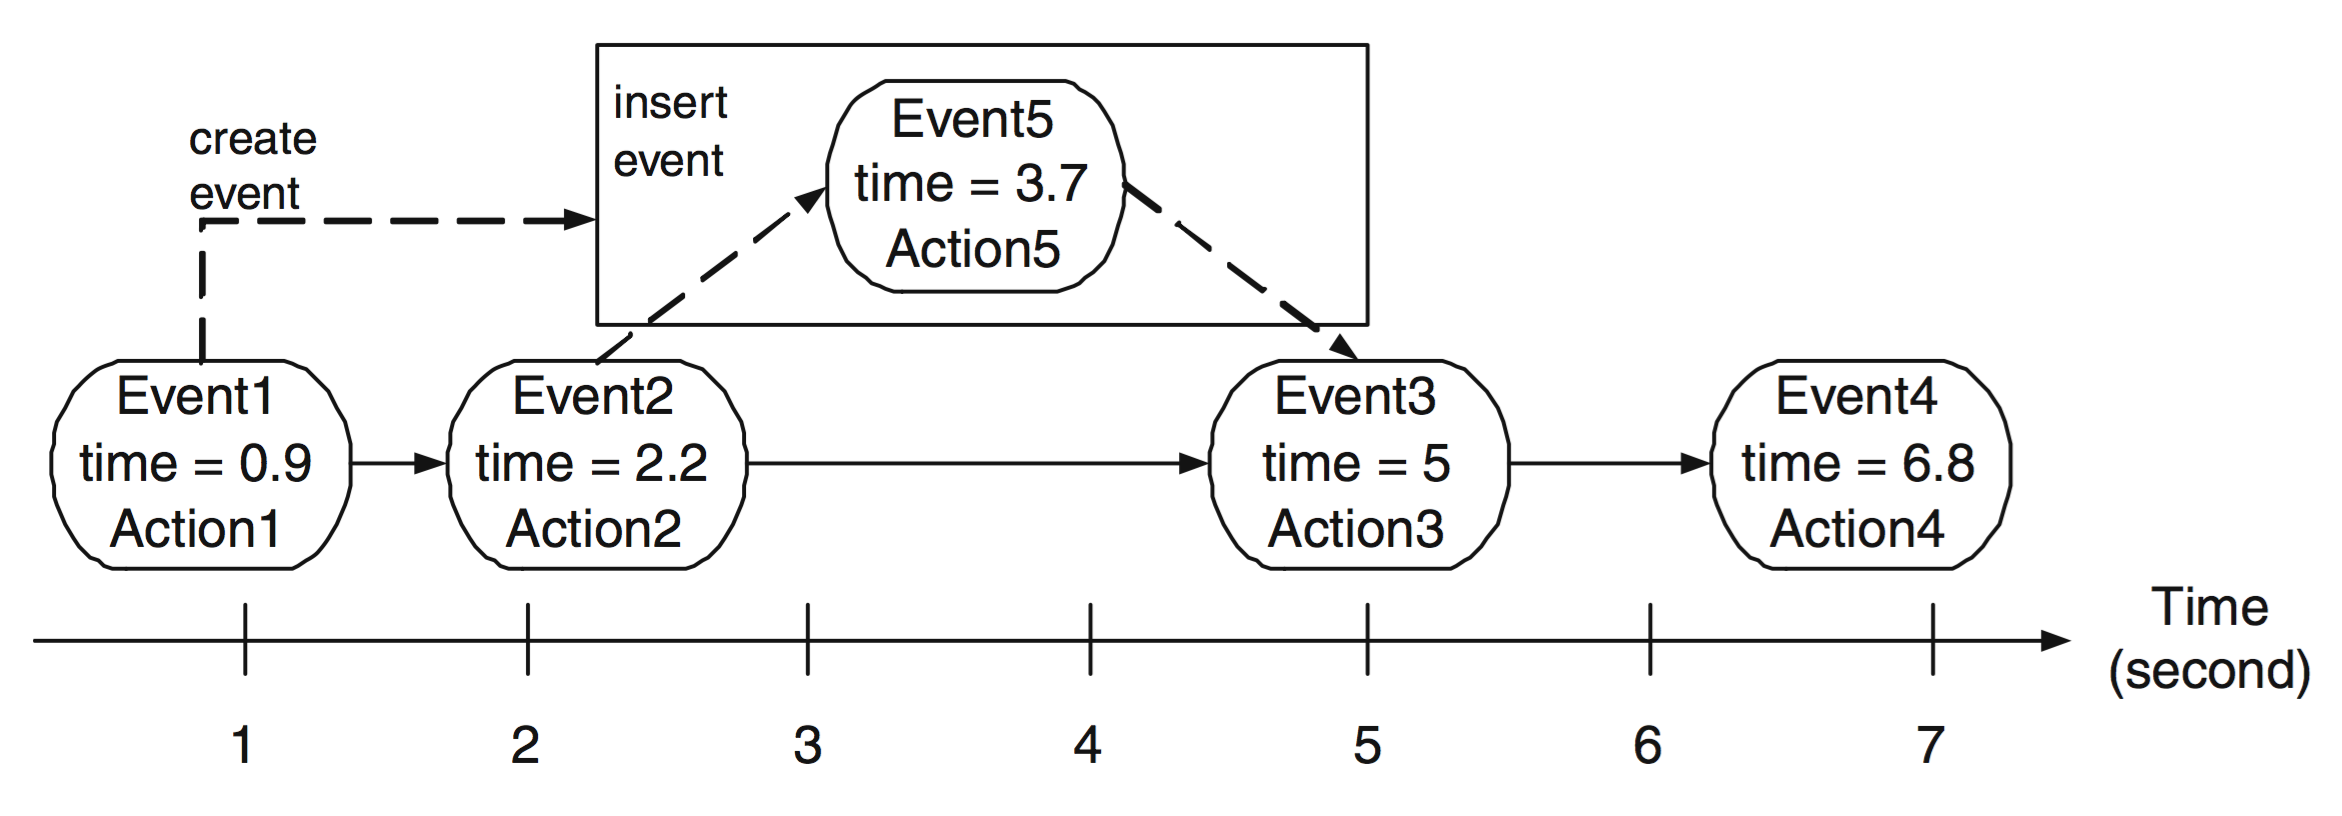
\includegraphics[width=0.6\textwidth]{Chapter5/Chapter5Figs/fig-ns2-event.png}
\caption{An example of event-chain in \emph{ns-2}.}
\label{fig-ns2-event}
\end{figure}

\section{WisSim Client}
\emph{WisSim} client is a software in the \emph{WisSim} toolkit which targets to have users create a network topology and analyze its properties. WisSim client consists of three main feature: WisSim Editor, WisSim Visualizer and WisSim Analyzer. In this section, we describe our addition features and improvements for WisSim client software. 
\subsection{Functional requirements}
\begin{table}[!htb]
\centering
\caption{Functional requirements}
\label{table-function-require}
\begin{tabular}{|p{2cm}|p{2cm}|p{2cm}|p{3cm}|p{2cm}|}
\cline{1-5}
Function        & Condition       & Input     & Output                                         & Module        \\ \cline{1-5}
Voronoi Diagram & Working project & Node list & Display                                        & WisSim Editor \\ \cline{1-5}
Graph           & Working project & Node list & Shortest path computed from Dijkstra algorithm & WisSim Editor \\ \cline{1-5}
\end{tabular}
\end{table}
\subsection{Class design}

\begin{table}[!htb]
\centering
\caption{Packet list.}
\label{table-class-design}
\begin{tabular}{|l|p{8cm}|}
\hline
Packet               & Implementation                                                                                                                                           \\ \hline
Graph/VoronoiDiagram & This packet contains implementation of Voronoi diagram construction algorithm and computational geometry library (such as line, point, circle, parabola) \\ \hline
Graph/Graph          & This packet implements primitive graph algorithms such as BFS, Dijkstra, ...                                                                             \\ \hline
\end{tabular}
\end{table}

\subsection{Screen design}
\begin{figure}[!htb]
\centering
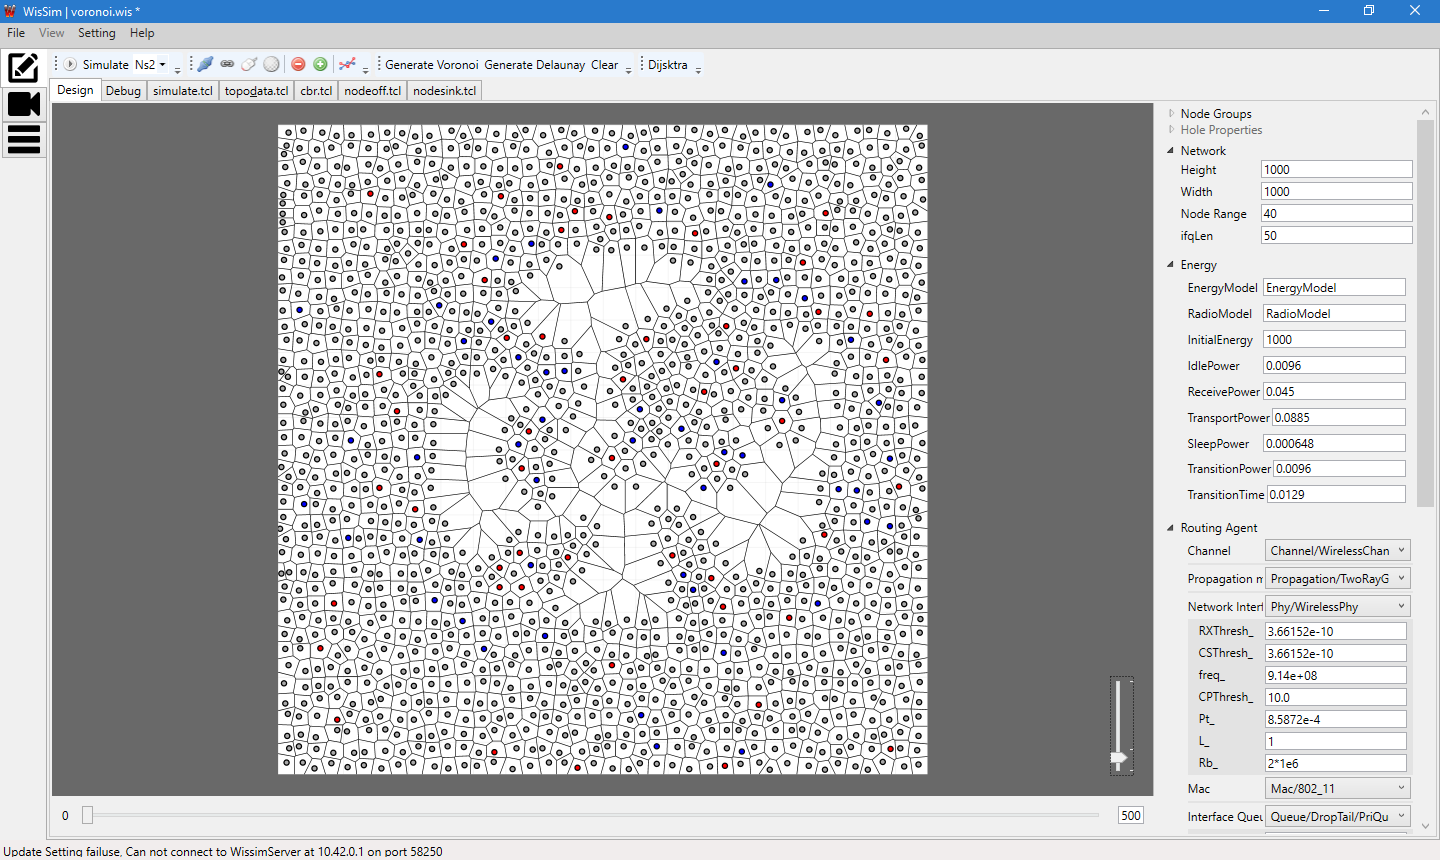
\includegraphics[width=0.8\textwidth]{Chapter5/Chapter5Figs/wissim-voronoi.png}
\caption{Screen of Voronoi diagram construction.}
\end{figure}

\begin{figure}[!htb]
\centering
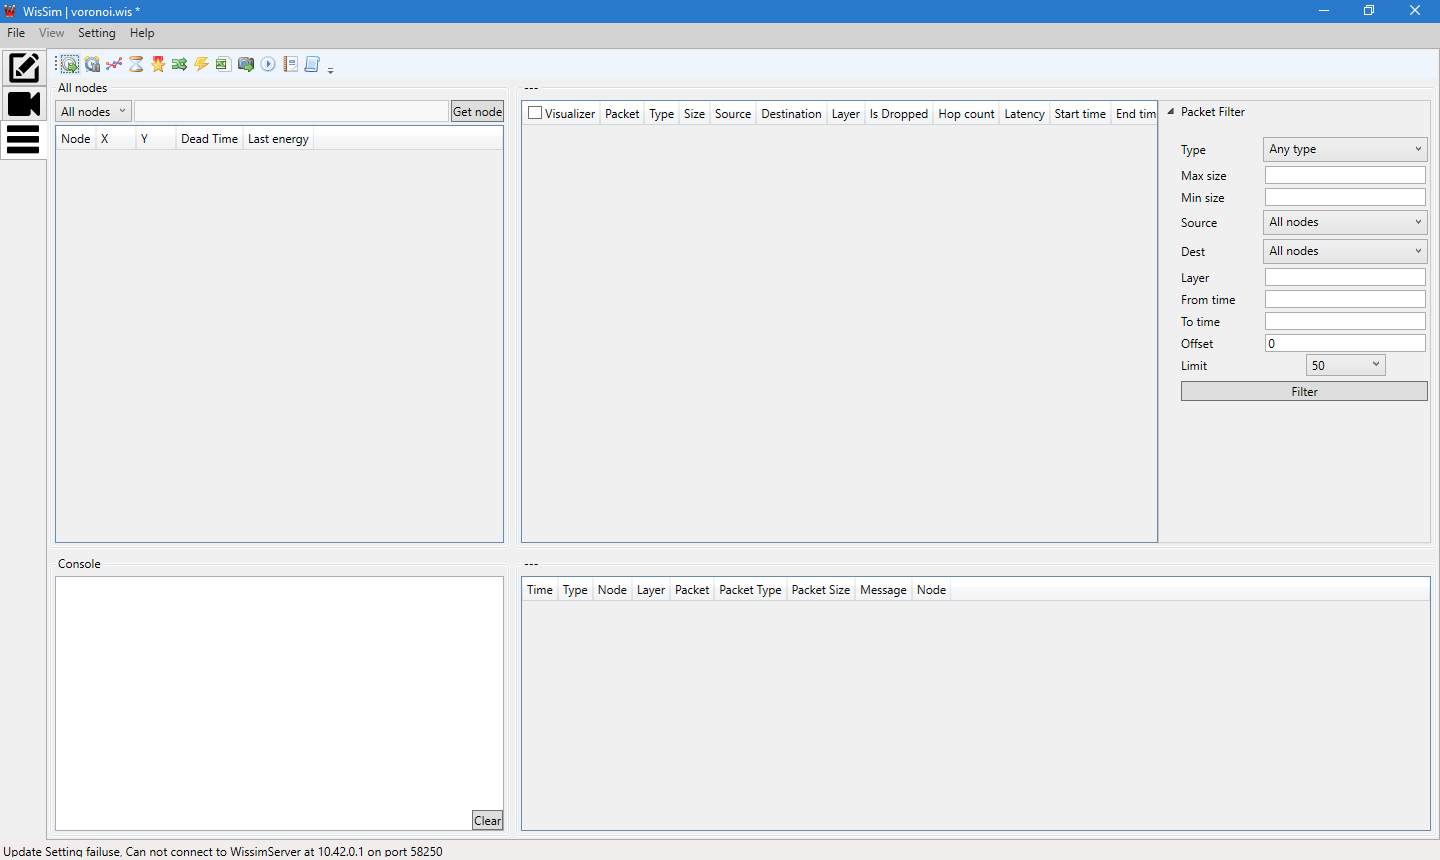
\includegraphics[width=0.8\textwidth]{Chapter5/Chapter5Figs/wissim-analyzer.png}
\caption{New design of WisSim Analyzer screen.}
\end{figure}